\chapter{相关技术综述}
本章主要介绍时下常用的漏洞挖掘技术,以及本系统将要用到的技术、工具和开发框架。

\section{漏洞挖掘技术}
漏洞挖掘指用自动化或半自动化技术对软件进行本身进行静态,动态分析,检测其是否存在安全漏洞的过程~\cite{liujian2018}。随着软件规模扩大,软件功能种类多样化,安全漏洞其种类也在不断增多,不同漏洞的产生原因不同,利用方式也不同,一种漏洞挖掘技术不能适用于所有漏洞,因此在实践中,人们会在软件开发的各个阶段应用不同类型的技术,本文将这些技术的应用场景主要分为三类:
\begin{itemize}
    \item  白盒测试:也成为静态测试,通常发生在软件编码阶段,对应用程序的源代码或对源码编译产生的二进制文件进行安全性审计,从而发现漏洞。该场景下的技术由于获取了源代码信息,也被称为源码扫描或静态扫描,其可以获得较高的代码覆盖率,发现更多的漏洞,但由于无法运行而产生大量误报,它也是本文系统的应用场景。
    \item 黑盒测试:通常发生在软件测试和运行阶段,对应用程序动态运行,并输入数据,分析程序反馈从而发现漏洞。适用于该场景的技术可以在程序只暴露接口的情况下展开测试,因此应用广泛,同时动态运行程序使其具有更低的误报,甚至产生漏洞利用报告,但由于如今应用程序复杂,自动化测试技术往往无法覆盖所有的代码逻辑。
    \item 灰盒测试:介于白盒和黑盒之间的一种测试,这一场景下的技术往往通过软件插桩或是逆向工程,不但关注程序输入输出信息,还可以了解部分程序内部逻辑。因此具备上述两种测试的优点,许多黑白盒测试技术稍加改造也可以变为灰盒测试技术,但由于其终究还是需要获取程序本身,以及需要动态运行,使用比纯黑百盒测试更为复杂。
\end{itemize}

在漏洞挖掘技术发展早期,每一种技术往往只能应用于一种特定场景,但随着研究者的不断完善和改进,如今一种技术也可以适用于多种场景,并且技术本身也产生了相互组合,对其正交分类较为困难,本章就目前常用的漏洞挖掘技术进行粗略分类并分别进行简要介绍~\cite{liujian2018,meihong2009}。


% 需要写java的常见漏洞吗?
\subsection{基于代码分析的漏洞挖掘技术}
这一类漏洞挖掘技术侧重于对程序代码本身进行分析,同时对漏洞产生原理进行建模,将程序分析结果结合漏洞模型发掘漏洞,主要用于白盒测试场景。主要有词法分析技术,数据流分析技术,形式化分析技术和符号执行技术。\\
\vspace{1cm}
\subsubsection{词法分析技术}
词法分析技术是最简单的一类漏洞挖掘技术,其主要思想是将代码文本与归纳好的缺陷模式进行匹配,以此发现漏洞。由于其不深入分析程序结构和语义,往往只能挖掘较为简单的一类漏洞,并且存在相当高的误报率,在实际场景下应用较少,但由于其思想简单,适用性很广,目前也还存在类似工具,如:MobSF~\footnote{\url{https://github.com/MobSF/Mobile-Security-Framework-MobSF}},Cobra~\footnote{\url{https://github.com/WhaleShark-Team/cobra}}。\\

\subsubsection{数据流和控制流分析技术}
数据流分析是一种按程序执行路径模拟数据流动的一种分析技术,其原本用于进行程序优化~\cite{Kildall1973},安全研究者们发现后将其运用于漏洞挖掘中,如今该技术在白盒,灰盒和黑盒测试都有应用~\cite{Shastry2016}。

在数据流分析过程中,存在过程内分析和过程间分析,过程内分析主要对函数内分析,而过程间的分析主要处理跨函数分析。
对于过程内分析,根据其对程序路径的分析精度,可分为流不敏感分析,流敏感分析和路径敏感分析。流不敏感的数据流分析只是按代码行号从上而下进行分析;流敏感分析会首先产生程序的控制流图(CFG, Control Flow Graph),再按照CFG的拓扑排序正向或逆向的分析;路径敏感信息不仅考虑到语句的先后顺序,还会考虑语句的可达性,即会沿实际可执行到路径进行分析。
过程间分析首先构造程序的调用图(CG, Call Graph),接着遍历图中的函数进行过程内分析,当遇到其他函数时,若已分析过,则直接使用分析结果向下分析,若未分析过,则跟进该函数,再次进行过程内分析,并且将分析结果保存。

数据流分析能够一定程度上理解程序语义,是一种比词法分析技术更为精确的一类分析技术,其关键在于准确的计算程序的数据流,此外,本文使用的污点分析技术作为数据流分析的一种特例,作为本系统所使用的技术之一,将在下文单独一章进行介绍。\\

\subsubsection{形式化方法分析技术}
形式化方法分析主要思想是将软件代码性质进行形式化描述,再判断该描述是否满足漏洞特征的一类分析方法~\cite{B:automatedTheoremProving},其中定理证明技术是形式化代码分析技术的主要代表。

%https://firmianay.gitbooks.io/ctf-all-in-one/doc/5.0_vulnerability.html
%Automated Theorem Proving in Software Engineering
%https://github.com/leanprover/lean2
定理证明技术将漏洞存在(或不存在)定义为一定理,再将源程序代码特征转化为数学表达形式,最后对数学表达进行逻辑推理,若定理存在性得以证明,则漏洞存在(或不存在),即漏洞挖掘过程类似于数学上的定理证明过程。主要代表性工具有 infer~\footnote{\url{https://fbinfer.com/}}~\cite{atp:infer}、 ESC/Java~\cite{atp:escjava} 和 saturn~\cite{atp:saturn}。

该技术作为一种使用严格的数理逻辑推理作为检测手段的技术,具有极低的误报率,但由于其需要针对特定漏洞构建数学条件,需要大量的人工参与,有的漏洞甚至难以用数学结构表达,导致其适用于死循环、资源泄露和空指针等问题,对新漏洞的扩展性不高,同时,如何将大规模程序应用于形式化方法分析也成为工业界亟待解决的问题。 \\

\subsubsection{符号执行技术}
符号执行技术是一种将程序执行可达性问题转化为约束求解问题,并以此进行漏洞挖掘的技术~\cite{sym:sum},代表性工具有angr~\footnote{\url{http://angr.io/}},DART~\cite{sym:dart}, CUTE~\cite{sym:cute}, EXE~\cite{sym:exe}和KLEE~\cite{sym:klee}。
% https://www.youtube.com/watch?v=mffhPgsl8Ws
% https://blog.csdn.net/wcventure/article/details/86773290
%Symbolic Execution for Software Testing: Three Decades Later

具体来说,符号执行包含一个符号状态表$\sigma$和一个符号路径约束$PC$,开始时,$\sigma=\empty, PC=true$,每读取一条语句,就将变量抽象为约束求解中的变量、常量或他们的表达式放入$\sigma$中,特别的,当遇到条件判断$if(e)$时,将if分支的$PC$更新为$PC \wedge \sigma(e)$,将else分支的$PC'$更新为$PC\wedge \neg\sigma(e)$,随后使用约束求解器求解$PC$和$PC'$,如果约束不满足,则停止对该分支的解析(因为该分支不可达)。当符号执行遇到程序崩溃、预先定义的漏洞语句、或是程序正常退出时,整个分析停止,同时可以计算可以到达停止点的输入。

符号执行可以分析程序中的控制流、覆盖更多的代码,同时也有效降低了误报率,但传统符号执行严重依赖于约束求解器的能力,例如,若约束求解器不能处理非线性计算,或是整个程序中存在无法分析的第三方库,那么整个分析将无法继续。为解决这些问题,研究者们提出了动态符号执行的想法~\cite{sym:dart,sym:cute,sym:exe,sym:klee},但其在实际应用中仍不是很广泛,主要原因在于其需要大量计算资源,甚至在处理大规模程序时,出现的路径爆炸问题会导致约束求解无法产生结果。\\

\subsection{基于模糊测试的漏洞挖掘技术}
模糊测试是一种通过构造大量非预期输入,同时观察软件运行反馈来发现软件漏洞的方法~\cite{fuzzingstateofart}。

由于其不需要了解程序内部具体实现,不论是Web应用还是二进制程序,其都是一种非常受欢迎的技术。
该技术的关键在于如何构造能够引发软件漏洞的输入,对于Web应用来说,扫描器会针对每个漏洞(如SQL注入,XSS等)准备若干个(或若干组)可能会引发漏洞的输入模式,接着爬虫程序会爬取网站所有URL(或是将URL也作为模糊输入的一部分),将输入模式整合进HTTP报文中并发送给服务器,若服务器返回符合漏洞特征(也被称为测试断言,Test Oracle),则报告程序存在漏洞,主要的工具有AWVS~\footnote{\url{https://www.acunetix.com/vulnerability-scanner/}},Netsparker~\footnote{\url{https://www.netsparker.com/}}和ZAP~\footnote{\url{https://www.zaproxy.org/}}。

学术界更热衷于对二进制程序的模糊测试技术进行改进~\cite{artoffuzz},为了构造能够到达更深层代码的输入,研究者们提出了基于变异的模糊测试和基于生成的模糊测试~\cite{Zou2018},基于变异的模糊测试通过当前模糊测试结果反馈和结合程序特征,对输入进行各类变异,以此指导测试方向,该方向主要有:代码覆盖率制导的模糊测试技术,如 AFL~\footnote{\url{http://lcamtuf.coredump.cx/afl/}}和libFuzzer~\footnote{\url{https://llvm.org/docs/LibFuzzer.html}};由符号执行制导的模糊测试技术,如 Driller~\cite{Driller}和由信息流制导的模糊测试技术,如 VUzzer~\cite{VUzzer}。基于生成的模糊测试技术适用于输入具有一定模式的场景,例如 PDF 阅读器,程序编译器或解析器等,例如 CodeAlchemist~\cite{CodeAlchemist} 即设计了一套 JavaScript 代码生成工具,以此发现 JavaScript 解释器的漏洞。

模糊测试作为一种能够得到漏洞利用输入的一种漏洞挖掘技术,在黑盒和灰盒场景下应用广泛,但由于目前程序日益复杂,该漏洞挖掘技术很难测试隐藏在复杂状态已经条件分支下的代码块,导致程序覆盖率不高,即其具有低误报,高漏报的特点。

\section{污点分析}
%https://www.k0rz3n.com/2019/03/01/%E7%AE%80%E5%8D%95%E7%90%86%E8%A7%A3%E6%B1%A1%E7%82%B9%E5%88%86%E6%9E%90%E6%8A%80%E6%9C%AF/
%https://github.com/firmianay/CTF-All-In-One/blob/master/doc/5.5_taint_analysis.md
%http://www.jos.org.cn/html/2017/4/5190.htm
%http://www.jos.org.cn/html/2019/2/5581.htm
污点分析属于数据流分析的变种,通过判断关键操作的数据(如调用危险函数的参数)是否可被用户操控,推测程序是否存在 安全性漏洞~\cite{taint:wanglei}。由于其了解程序上下文,并且有较强的可解释性——安全工程师可以通过跟踪污点传播过程判断是否存在安全问题,因此其也成为了挖掘 Web 或 Android 漏洞较为常用的技术,也被很多开源或商用白盒扫描器使用,如:Pixy~\cite{pixy}、Find Security Bugs ,Fortify~\footnote{\url{https://www.microfocus.com/en-us/solutions/application-security}}和LGTM~\footnote{\url{https://lgtm.com/}}。\\

\subsection{污点分析原理}

\subsubsection{污点分析三要素}
污点分析主要有三个组成要素:污点信息的产生点(source)、污点信息的汇聚点(sink)和污点信息的清洁点(clean),它们通常需要富有经验的安全工程师手动设置。

\begin{itemize}
	\item 产生点(Source):污点的产生点往往是用户输入的数据,比如Web应用中读取URL参数的函数,顾名思义,这些函数调用后的返回值被标记为污点——攻击者可以操控的数据点。
	\item 汇聚点(sink):检查点是程序的一些敏感操作,如调用数据库查询语句,或是将数据返回到网页,如果这些操作的操作数据是污点,那么意味着操作可被攻击者利用,即程序存在漏洞。
	\item 清洁点(clean):清洁点通常是对污点进行消除的一类操作,如SQL注入、XSS中的过滤函数。清洁点是污点传播准确性的重要保证,不能识别清洁点即会引发污点过污染问题。
\end{itemize}


\subsubsection{污点分析过程}         
污点分析分为静态污点分析和动态污点分析,两者区别在于静态污点分析只使用程序代码模拟污点传播过程,而动态污点传播则通过程序的实际运行进行传播,由于本文关注于白盒测试情景,故只介绍静态污点传播方法,而在下一子章节会介绍动态传播的优劣势。

在定义好三要素之后,污点分析法会与数据流分析一样,对程序进行过程内分析和过程间分析。

过程内分析包括了显式流分析和隐式流分析,显示流分析即通过分析变量的数据依赖关系进行污点传播,而隐式分析则是指考虑控制依赖进行污点传播。

\begin{figure}[!htbp]
	\centering
	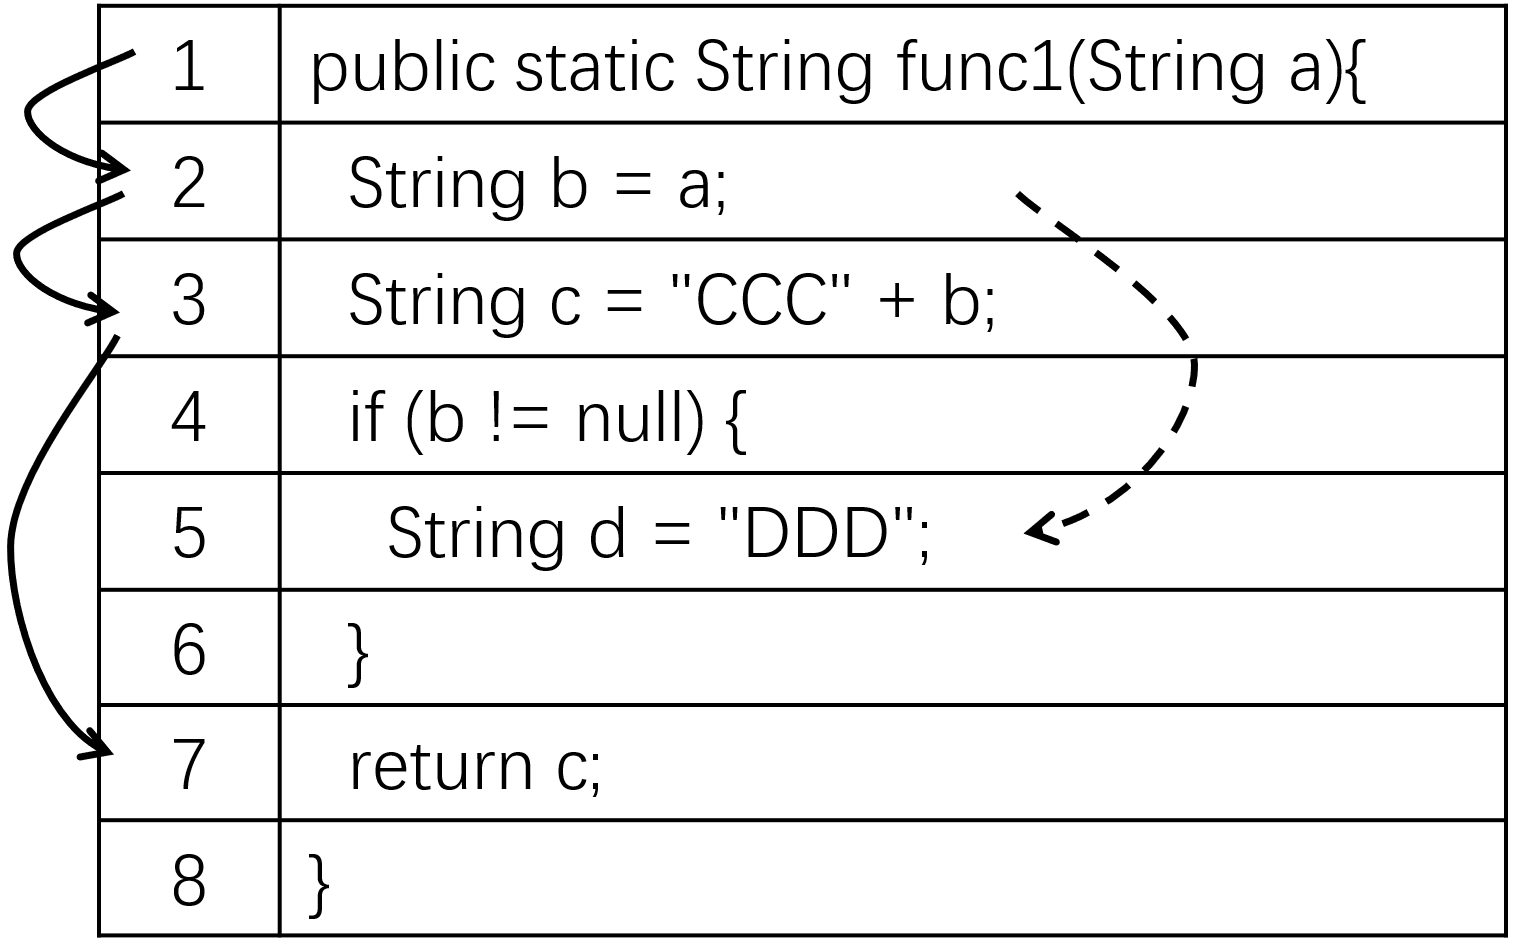
\includegraphics[width=0.5\linewidth]{FIGs/chapter2/internal_taintflow.png}
	\caption{过程内污点分析}\label{internalflow}
\end{figure}

如图~\ref{internalflow}所示,首先假设变量$a$为污点变量,实线箭头表示了显示污点传播路径,而虚线箭头表示了隐式污点传播路径,同时该图也说明了过程内污点传播基本思想,即从上至下遍历数据流图,若未标记的变量依赖于污点变量,则新变量也被标记为污点变量。虽然攻击者确实可以利用控制依赖操作数据进行攻击,但由于其分析复杂且会产生大量误报,在工程领域常常只做数据流依赖的显示分析,因此本文主要讨论显式流分析。

现代程序存在着复杂的函数调用,除了进行过程内分析,还需要进行过程间分析。其分析首先构造函数调用图(Call Graph),接着搜索存在产生点的函数,对于每一个存在产生点的函数,自顶向下分析(也可以自底向上分析)。遇到函数调用时,跟进被调函数,进行过程内污点分析,将分析结果表达为$\left\langle f, S, r\right\rangle$的函数摘要,其中$f$包含函数本身摘要信息(类名方法名和函数签名),$S$指调用过该函数后被污染的变量集合,$r$取值0或1,标记函数返回值是否被污染;接着根据函数摘要,再进行过程内分析,如此往复直至分析完函数所有代码块或是污点传播至汇聚点,报告漏洞。

\begin{figure}[!htbp]
	\centering
	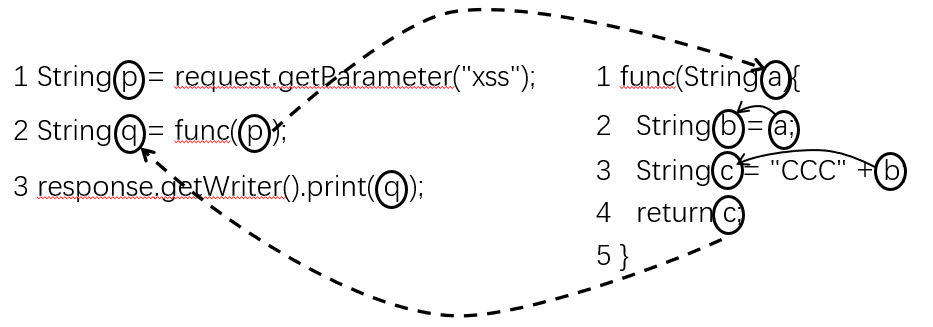
\includegraphics[width=0.7\linewidth]{FIGs/chapter2/external_taintflow.png}
	\caption{过程间污点分析}\label{externalflow}
\end{figure}

如图~\ref{externalflow}所示,分析过程从左侧函数开始,因为其找到了一处产生点——\textit{request.getParameter("xss")},于是将污点传递到变量\textit{p},接着调用函数\textit{func(p)},于是对函数\textit{func}做过程内分析,得到其函数摘要,$\left\langle func, \left\{a, b, c\right\}, 1\right\rangle$,于是回到调用者的函数内,变量\textit{q}被标记为污点,又因为第三行存在一处汇聚点——\textit{response.getpriter.print()},并且参数为污点,于是报告此处有漏洞,并且根据汇聚点可以判断该漏洞是一个 XSS 漏洞。\\

\subsection{污点分析的优势和不足}
污点分析能够对程序上下文有一定理解,往往能产生误报率相对较低以及可解释的漏洞报告,其方法对 Web 类型的安全漏洞覆盖率较高,而污点类型的漏洞普遍具有较高的危害性~\cite{taintStyle,aletheia},因此该方法已被很多工业界、学术界的安全静态扫描工具所使用~\cite{taintStyle,taint:taj,pixy},本文也选择该技术产生初步的漏洞扫描结果。

然而,污点传播仍有可能发生误报,以下通过简单示例来说明。

\begin{figure}[!htbp]
	\centering
	\subfigure[污点传播难以处理容器类型]{
		\label{taintcase1}
		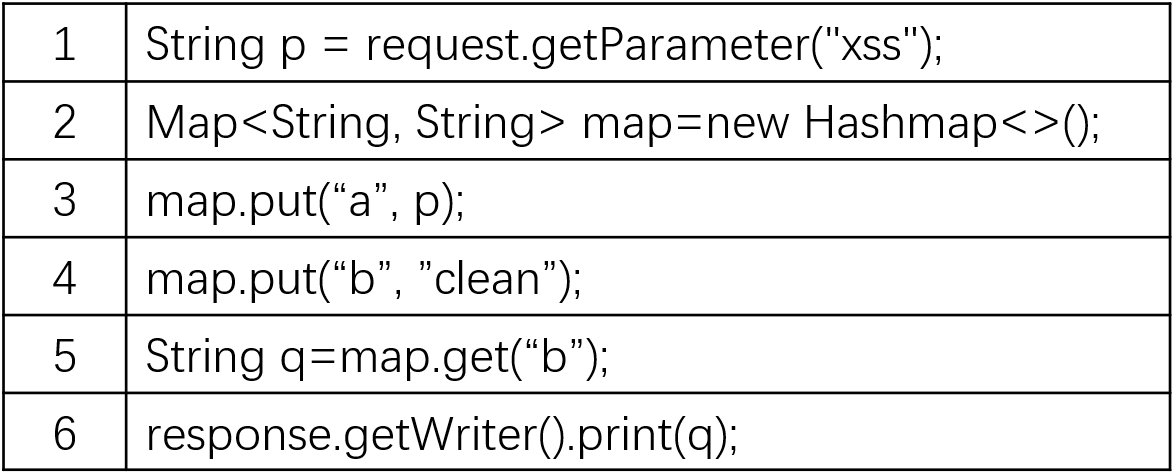
\includegraphics[width=0.4\textwidth]{FIGs/chapter2/tpcase1.png}}
	% \hspace{0.1in}
	\subfigure[污点传播难以分析控制流]{
		% \label{fig:subfig:b} %% label for second subfigure
		\label{taintcase2}
		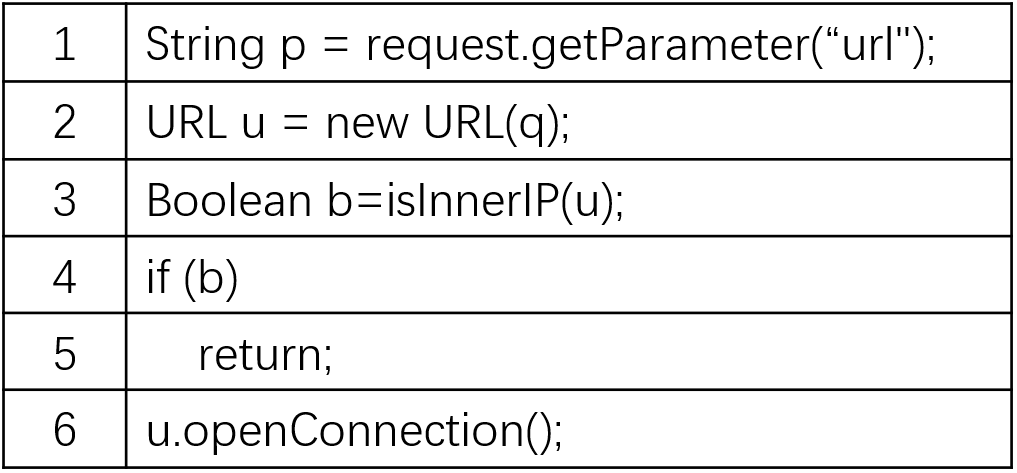
\includegraphics[width=0.4\textwidth]{FIGs/chapter2/tpcase2.png}}
	\subfigure[污点传播难以处理特殊污染条件]{
		% \label{fig:subfig:b} %% label for second subfig ure
		\label{taintcase3}
		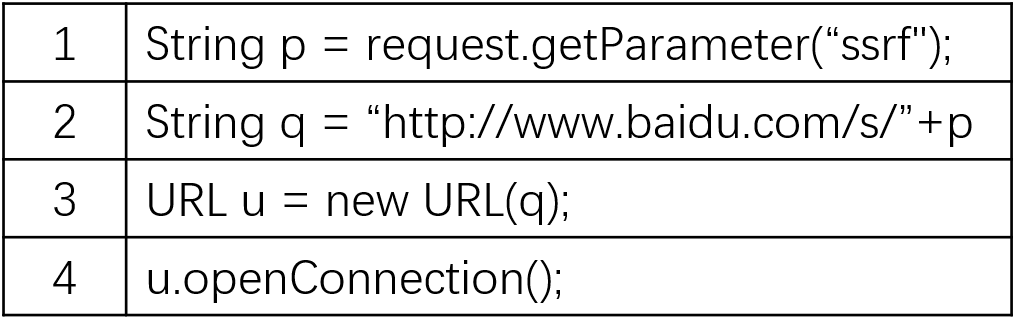
\includegraphics[width=0.4\textwidth]{FIGs/chapter2/tpcase3.png}}
	\subfigure[污点传播难以分析清洁函数]{
		% \label{fig:subfig:b} %% label for second subfigure
		\label{taintcase4}
		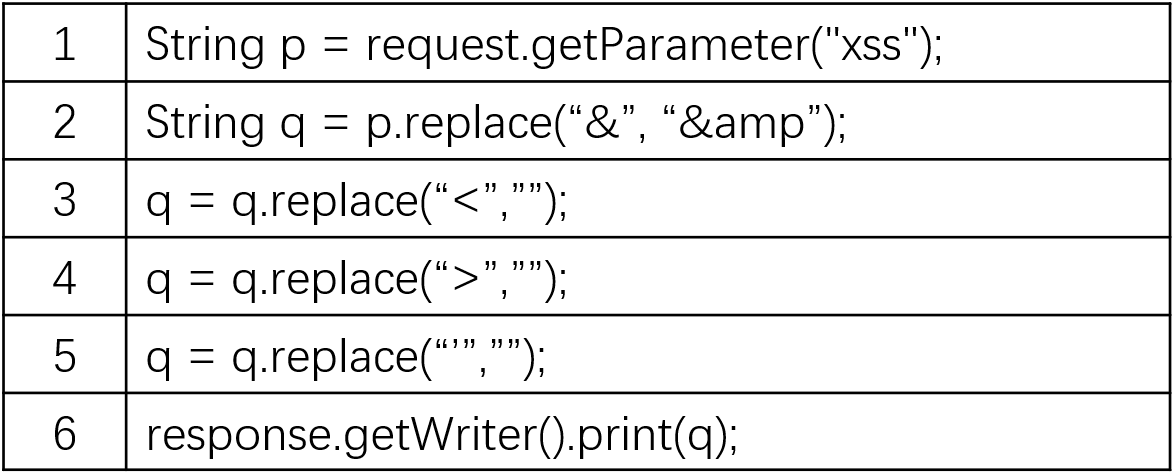
\includegraphics[width=0.4\textwidth]{FIGs/chapter2/tpcase4.png}}
	\caption{污点传播的不足}
	\label{fig:rq3} %% label for entire figure
\end{figure}
首先,污点传播对容器类型无法做很好处理,如图~\ref{taintcase1}所示,当污点传入容器类型时(在此例子中为\textit{map}),静态污点传播只能将这类变量的传播规则设为传播/不传播污点,从而造成过污染/欠污染,就如图所示,若设为\textit{map}传播污点,由于案例实际从容器中取出的是没有污点的变量,即过污染,而若设为不传播,若\textit{q}取出了参数\textit{p},那么又导致了欠污染。动态污点传播虽然解决了这一问题,但是由于其使用条件复杂,且无法用于静态分析,本文暂不讨论。

此外,静态污点传播对控制流没法做很好的处理,如图~\ref{taintcase2}所示,在第三行,程序已经对可能产生的 SSRF 漏洞进行了处理,即如果是内部地址的话则直接返回,但是不论是考虑显式流还是隐式流,污点传播都不能避免这一类误报。

再者,对于特殊触发条件的漏洞,污点传播无法很好处理,如图~\ref{taintcase3}所示,在第二行,因为 SSRF 要求攻击者能够操控主机名,所以即使用户输入的污点变量拼接在了一个正常网站之后,程序也不会出现 SSRF 的问题,而按照污点传播分析法,毫无疑问它会报告这段程序存在SSRF漏洞。

最后,不论是动态污点传播还是静态污点传播,其对污点清洁点的识别能力几乎为零,如图~\ref{taintcase4}所示,程序已经对潜在的XSS攻击做出的处理——即在第2$\sim$5行对用户输入的特殊符号进行替换和过滤,但是污点传播并不能识别这些清洁点,导致误报。    

正是因为存在这些不足,本文将在下文引入程序切片技术和 BLSTM 来降低误报率。\\

\subsection{Java污点分析工具选型}
Java上的污点分析工具有很多,如 Find Security Bugs,TAJ~\cite{taint:taj}。但对于安全扫描工具来说,除了污点传播引擎,针对漏洞定义好大量的入口点和汇聚点是扫描低漏报的重要保证。Find Security Bugs 作为较为经典的扫描工具,前人已经为预先定义了大量的污点传播入口点和汇聚点,并且支持自定义新的入口点和汇聚点,非常适合二次开发。

本系统保证准确性的手段在于利用机器学习对污点传播的误报进行改进,而不是定义大量污点传播规则,因此本文使用 Find Security Bugs 进行污点传播分析。此外,本系统解决了原版 Find Security Bugs 不能展示传播路径的问题,使其更加易用。\\

\section{程序切片技术}
\subsection{程序切片定义}
% https://www.cnblogs.com/maifengqiang/archive/2013/05/21/3090739.html
% https://hacpai.com/article/1555083057303
% 前向切片与后向切片之间关系的研究.pdf
程序切片技术是一种通过对程序分析,抽取程序中与关注点相关的一组语句集合的技术,目前广泛运用于程序调试,程序测试,优化,安全分析等领域。

该技术首次由Mark Weiser在其博士论文中提出~\cite{slices:weiser1979},他将程序切片做了如下定义:

将程序抽象为图$G\langle N,E\rangle$,$N$为程序中的语句集合,$E$为$\left\langle n,m \right\rangle$的集合,其中$n$为数据流的上一条语句,m为数据流的下一条语句。

\begin{definition}[程序状态序列(state trajectory)]
    
    若程序$P$中有长度为$k$的程序状态序列$T$,则:
    $$T=\left\langle \left\langle n_{1},s_{1} \right\rangle, \left\langle n_{2},s_{2} \right\rangle , \cdots , \left\langle n_{k},s_{k} \right\rangle \right\rangle$$
    其中$n_{i} \in N$,$s_i$为一个单射函数,记录所有变量到具体值的映射。
\end{definition}

\begin{definition}[切片准则(Slicing citerion)]
    
    若对于程序$P$有切片准则$C$,则$C=\left\langle i, V \right\rangle$,其中$i$指关注点,通常是指一条程序语句,$V$表示程序$P$中的变量子集(通常为$i$上的变量集合)。
    
\end{definition}

该切片准则决定了一个投影函数$Proj_C$:
$$
\operatorname{Proj}_{\langle i, V\rangle}(T)=\langle\operatorname{Proj}_{(i, V)}^{\prime}\left(t_{1}\right) , \cdots, \operatorname{Proj}_{\langle i, V\rangle}^{\prime}\left(t_{n}\right) \rangle
$$
其中:
$$
\operatorname{Proj}_{\langle i, V\rangle}^{\prime}(\left\langle n, s \right\rangle)=\begin{array}{ll}
{\lambda} & {\text { if } n \neq i} \\
{\langle n, s | V \rangle} & {\text { if } n=i}
\end{array}
$$
其中$\lambda$指空字符串,$s|V$指$V$中变量的单射函数。上式的含义是指,切片准则让我们只考虑$V$中变量的状态序列,并且只有当语句是关注点时,函数才返回状态序列,否则返回空字符。

\begin{definition}[程序切片]
    
    切片$S$为一组源程序语句的子集,它由不停地删除零条或多条原程序语句得到,同时保证$\operatorname{Proj}_{C}(T)=\operatorname{Proj}_{C^{\prime}}\left(T^{\prime}\right)$其中$T'$指切片中的状态序列,而$C'=\langle succ(i), V \rangle$,$succ(i)$指最靠近关注点$i$的语句(如果V不是$i$上的变量集合)或者就是$i$本身(如果$ V $是$i$上的变量集合)。
    
\end{definition}

按照定义,可以知道Mark Weiser实际上定义的是后向切片(backward slices),即切出对关注点造成影响的所有语句和谓词集合。对其改进后也出现了前向切片(forward slices),即切出被关注点影响的其他语句和谓词集合。\\

\subsection{程序切片技术}
%https://www.cnblogs.com/maifengqiang/archive/2013/05/21/3090739.html
程序切片技术自诞生以来,也经历了多个阶段~\cite{slices:xu2005brief},起初为Mark Weiser的概念阶段,主要通过控制流来进行程序切片;随后发展为基于依赖图的切片阶段,Ottenstein等人~\cite{slices:ottenstein1984program}首先提出了运用程序依赖图(PDG,Program Dependence Graph)进行切片,主要思想是首先对程序建立程序依赖图,再通过对程序依赖图的可达性计算进行后向切片,程序依赖图是一种反应语句数据依赖和控制依赖的一种程序中间表达形式,图中的点为单条程序语句,而图中的边则表示语句之间存在数据依赖关系,例如图~\ref{internalflow}的代码中,第三行与第二行就存在数据依赖关系,第七行与第四行则存在控制依赖关系。PDG只适用于单个函数的切片,horwitz等人~\cite{slices:horwitz1990}提出了系统依赖图(SDG, System Dependence Graph)的概念,在 PDG 的基础上,额外增加了两种边,一种边表示调用函数和被调用的直接依赖关系,另一种边描述由于边的依赖而引发的间接依赖关系,同时,前向切片也在此阶段产生;第三阶段为面向对象程序切片阶段,研究者提出将接受对象作为一个隐藏参数,结合多态解析手段,将面向对象切片问题转换为一般切片问题,使程序切片可以运用于面向对象语言。

目前已有很多工具可以对java程序进行切片,例如WALA(T.J. Watson Libraries for Analysis)~\footnote{\url{http://wala.sourceforge.net/wiki/index.php/Main_Page}}和Joana~\footnote{\url{https://pp.ipd.kit.edu/projects/joana/}}。WALA原本由IBM T.J. Watson 研究中心作为DOMO项目的一部分进行开发,在2006年,IBM将改软件转赠给社区。其主要功能包括Java类型系统和类层次分析,过程间数据流分析、指针分析和调用图构造以及上下文相关的切片等。Joana是由卡尔斯鲁厄理工学院推出,基于WALA 的一些分析手段构造的另一款 Java 切片工具,其包含指针分析,异常分析和PDG构图等复杂功能,并且其切片结果中能够更清晰的看到函数调用时实参的值,而对于污点传播类型中的自定义过滤函数,实参的值是一个很重要的特征(见图~\ref{fig:sliceresult}),因此本文选择Joana作为程序的切片器。\\
\begin{figure}[!htbp]
	\centering
	\subfigure[目标程序]{
		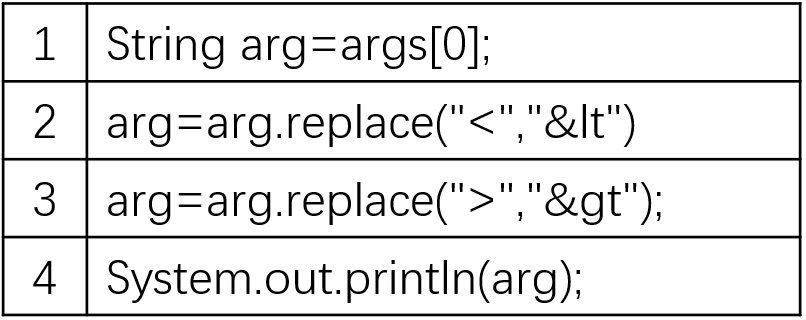
\includegraphics[width=0.4\textwidth]{FIGs/chapter2/slicetarget.png}}
	% \hspace{0.1in}
	\subfigure[Joana程序切片结果]{
		% \label{fig:subfig:b} %% label for second subfigure
		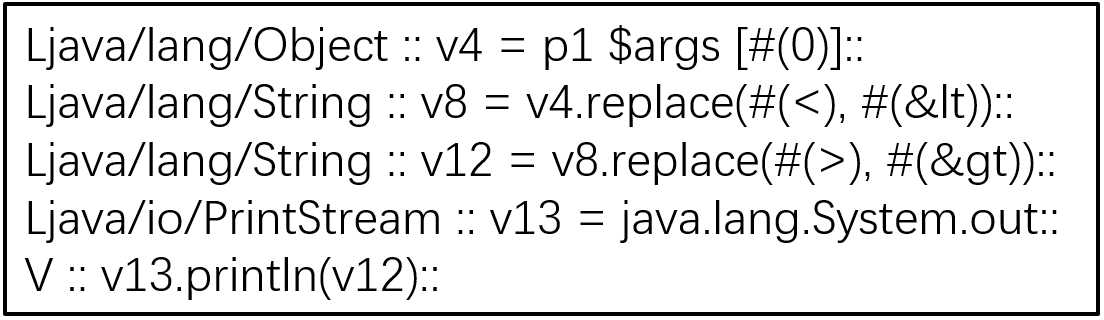
\includegraphics[width=0.4\textwidth]{FIGs/chapter2/joanaslice.png}}
	\subfigure[WALA程序切片结果]{
		% \label{fig:subfig:b} %% label for second subfigure
		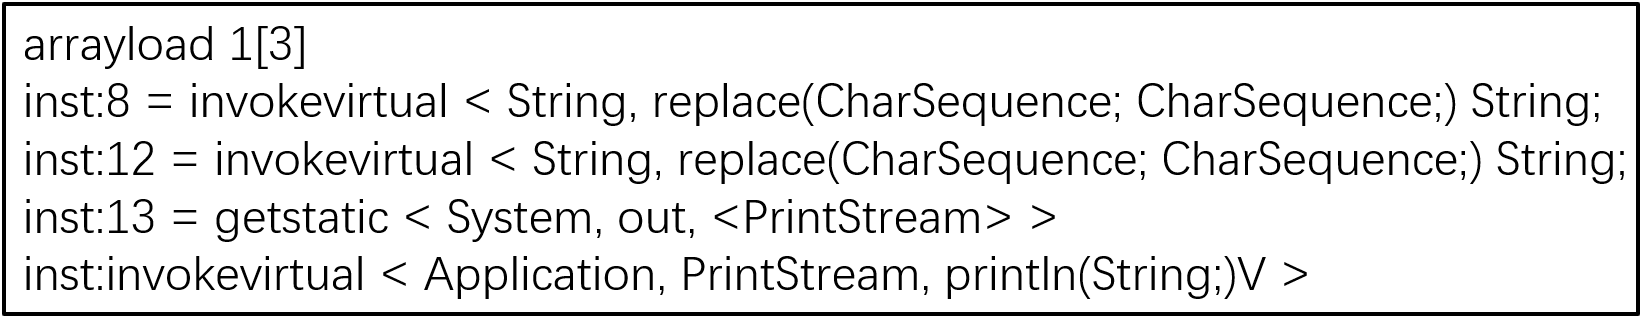
\includegraphics[width=0.85\textwidth]{FIGs/chapter2/walaslice.png}}
	\caption{Joana和WALA程序切片示例}
	\label{fig:sliceresult} %% label for entire figure
\end{figure}

\subsection{后向程序切片的优势与不足}
程序切片能够得到影响关注点的程序语句,在有效缩短了程序上下文、降低被分析代码量的同时,还能有效保留控制流的信息,在程序调试,软件度量或是软件安全中已经得到了很广泛的应用。

由于污点传播已经对程序由上而下的进行了分析,通过对汇聚点和污点值进行后向程序切片,可以从反方向分析漏洞代码,暴露先前没有考虑的控制语句,同时通过进一步的特征处理,可以作为神经网络的输入,弥补污点传播对控制流分析不足的缺陷,因此本文采用该技术作为特征处理的基础工作,另外由于程序切片属于较为传统的技术,在java语言上已有较为成熟的工具,考虑到 Java 漏洞的特征与函数参数强相关这一特性,本文选择 Joana 进行程序切片。

然而,传统后向程序切片也存在不足,目前最大的挑战在于当程序规模变大时,后向程序切片效率低下;此外原生 Joana 并不支持在缺失程序依赖下对其程序进行切片,而在 SCA 的输入中,缺失依赖的程序又是非常常见的,针对以上问题本文做出了分段切片、限制调用图切片和无依赖切片的技术调整,具体细节将在第三四章节详细说明。\\

\section{BLSTM算法}
双向长短期记忆网络(BLSTM,Bidirectional Long Short-Term Memory)是一种特殊的循环神经网络(RNN,Recurrent neural network),主要改进有双向读取和增加记忆门两方面,是一种在自然语言处理上应用广泛的神经网络~\cite{lstm:translate}。\\

\subsection{LSTM原理介绍}
为了保证在不同的序列数据上,相同数据点有不同输出结果,人们将其记忆体加入神经网络之中,从而产生了RNN,然而RNN在处理较长文本时,存在着梯度爆炸或梯度消失的问题~\cite{lstm:gradient},Hochreiter和Schmidhuber于1997年在记忆体中加入写入、输出和遗忘门,而改进后的神经网络也被成为长短期记忆网络(LSTM,Long Short-Term Memory)~\cite{lstm:1997}。

\begin{figure}[htb]
	\centering
	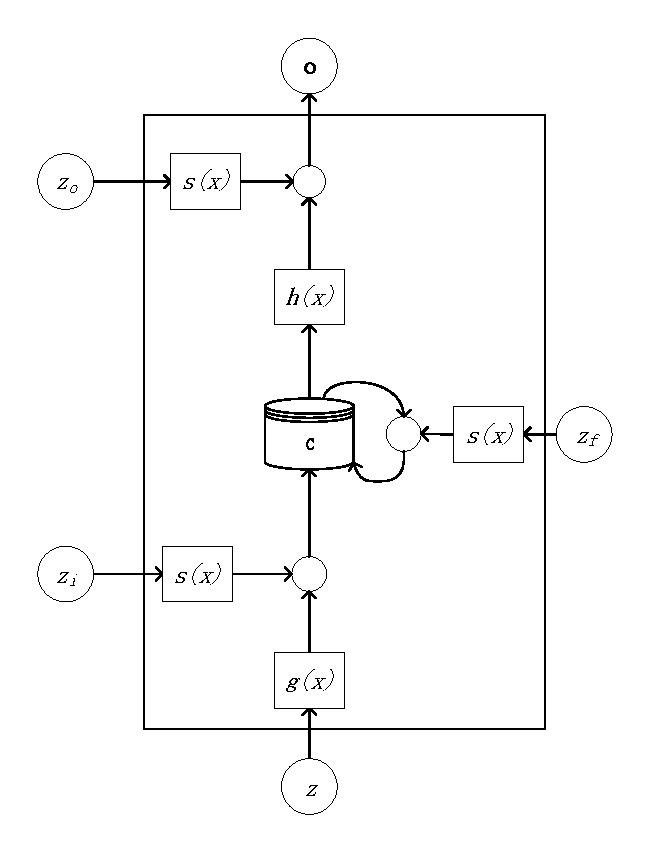
\includegraphics[width=0.4\linewidth]{FIGs/chapter2/lstm_cell.pdf}
	\caption{LSTM的神经元}\label{lstmcell}
\end{figure}
如图~\ref{lstmcell}所示,一个LSTM的神经元有四个输入:$z$表示原输入,$z_i$表示输入门,$z_f$表示遗忘门,$z_o$表示输出门,以及有一个输出$o$,神经元内有一记忆体$C$,在下一时刻的输入进入神经元时,记忆体下一时刻的值$C'=g(z)*s(z_i)+C*f(z_f)$,$g(z)$为输入值的激活函数,$s(z)$为门限的激活函数,通常取sigmoid函数,从公式可以看出,首先输入门控制了输入数据本身是否可以输入进神经元,接着遗忘门控制了记忆体中旧数据是否会保留,最后输出$a=tanh(c')*f(z_o)$,显然,$z_o$控制了记忆体是否向外输出。

\begin{figure}[htb]
	\centering
	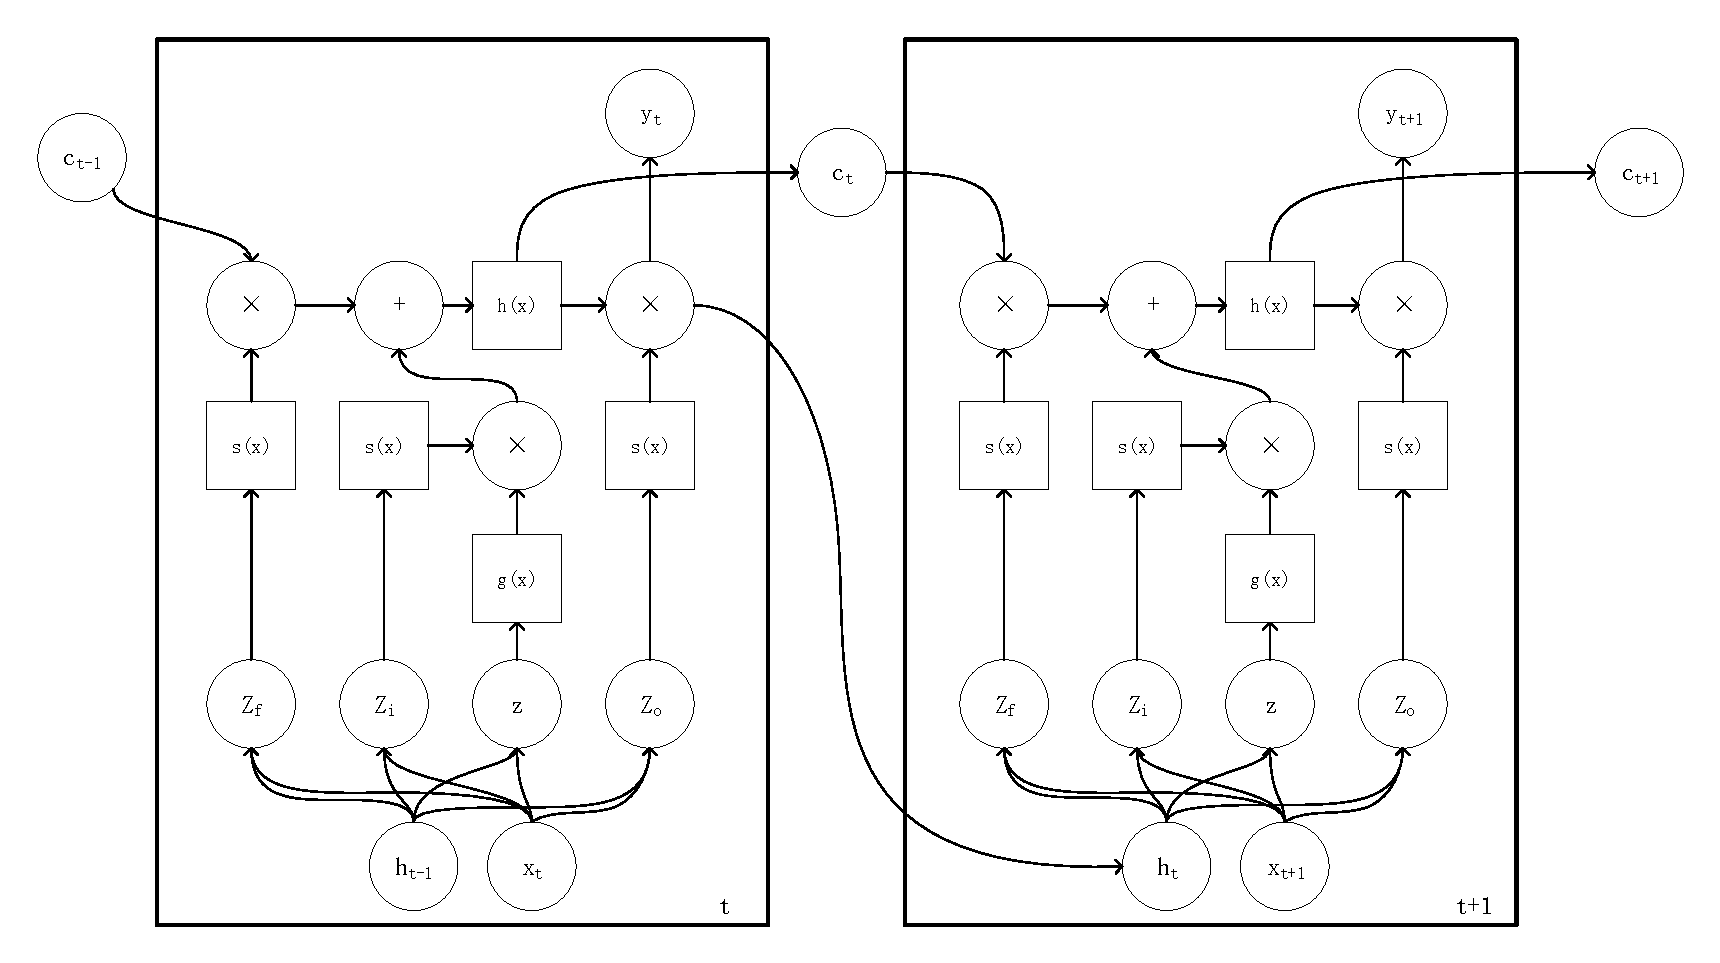
\includegraphics[width=0.8\linewidth]{FIGs/chapter2/lstm_time.pdf}
	\caption{LSTM的处理时序数据示意图}\label{lstmtime}
\end{figure}

利用LSTM处理时序数据情况如图~\ref{lstmtime}所示,对于任意时刻$t$,有$h_{t-1}$和$c_{t-1}$($t_0$时为随机值),$h_{t-1}$和$x_t$通过线性变换得到$z_f$、$z_i$、$z$和$z_o$,例如,$z_f=W_{f}\times [h,x]+b_{f}$。$z_f$、$z_i$、$z$和$z_o$均为以为向量,其长度等于该层LSTM神经元的个数,按上文所述,这4组向量输入神经元,结合神经元内的记忆体$c_{t-1}$计算得到输出$y_t$,同时$y_t$的值也作为下一轮输入的一部分,即$h_t$。$h_t$和$x_t+1$作为下一时刻的输入,输入下一时刻的神经元。在自然语言处理领域,人们通常利用最后一个时刻的输出对自然语言分类。\\

\subsection{双向读取——BLSTM}
早在RNN时期,就有研究者提出双向RNN提升拟合或预测准确性的思想,而LSTM作为RNN的一种,自然也可以运用该思想对其进行优化。

\begin{figure}[htb]
	\centering
	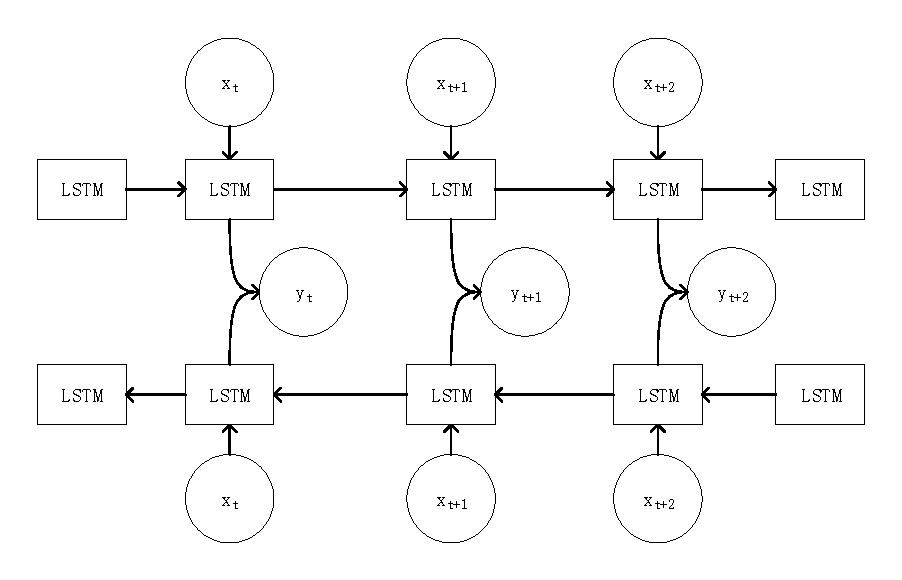
\includegraphics[width=0.8\linewidth]{FIGs/chapter2/blstm.pdf}
	\caption{BLSTM处理时序数据示意图}\label{blstm}
\end{figure}
如图~\ref{blstm}所示,对于一组时序数据$X=\left\{ x_0,\dots,x_t,x_{t+1},\dots,x_{k} \right\}$,训练两个LSTM网络,第一个网络正向读取数据(如图上方所示),第二个网络逆向读取数据(如图下方所示),在同一时刻,结合两个方向的网络输出值作为该时刻的输出(如果用于分类问题,通常结合正向$t_k$的输出和逆向$t_0$的输出)。


\subsection{BLSTM 的优势}

BLSTM的优势在于,单向LSTM在$x_t$时刻的输出实际上只被$x_0, x_1, \dots, x_t$影响,即其只能考虑截止到当前时刻的数据,而BLSTM的在某一时刻的输出值不仅受到该时刻正向数据的影响,还能受到该时刻后向数据的影响,因此有纵观全局的能力。\\

LSTM 增加了门限机制,解决了RNN 梯度爆炸或梯度消失的问题,而 BLSTM 通过双向传播机制,能够综合正向时序和逆向时序信息,是时序数据的分类和拟合问题(如自然语言处理问题)较为合适的算法。而目前已有很多利用自然语言处理和该模型进行程序分析的研究~\cite{naturalSoftware,lstm:recognize,lstm:repo,vuldeepecker,Koc2017,Koc2019}。所以本系统采用 BLSTM 作为污点传播预测算法,将污点传播的切片作为上下文敏感的自然语言数据,通过训练集训练 BLSTM 参数将其保存,在给定污点传播的切片输入时,系统调用训练好的模型对其进行预测。

\section{Django 框架}
\subsection{Django 框架简介}
Django 是一个高级的 Python Web 开发框架~\footnote{\url{https://www.djangoproject.com/}},它使开发者能够对 Web 应用进行简洁实用的设计并对其进行快速开发。Django 由一群有经验的开发者开发,其框架和内部设计避免了很多 Web 开发的问题,帮助开发者只关心于他们Web应用本身的逻辑而不需要重新开发通用组件。

Django 采用模型视图模板(MVT,Model-View-Template)模式,在模型层,其有一套高效的对象关系映射(ORM,Object Relational Mapping)框架和一些常用对象,比如用户对象,管理员对象等;在视图层,Django 阶级了基于正则表达式的URL分派系统,能够让用户灵活的处理自己的 URL 路由,并且内置的 Request,Response 对象能够让开发者快速的获取和返回数据;在模板层,Django 有自己的原生模板引擎,类似于 Jinja2,同时支持用户更换第三方引擎,保证用户充分自由的展现其数据。除此之外,Django 还内置了一个用户管理后台和各类安全保障模块,使大大加速了开发者的开发过程。\\

\subsection{Django 框架优势}
本系统的后台主要是对机器学习模型的操作,因此自然选择了 Python 开发语言,而 Django 作为 Python 语言上应用最为广泛的Web开发框架之一,自然也成为了本系统后台的首选技术。
利用 Django 的灵活性,本系统利用其 URL 分派系统接受客户端传来的预测、训练、标记等请求并对其处理,通过 ORM 框架将程序切片、模型训练数据快速本地化,以完成对系统后台的快速开发。

\section{本章小结}
本章首先介绍了目前流行的漏洞挖掘技术,并对其优劣势进行了说明,接着介绍了本系统使用的技术、工具和框架,并分别说明了使用这些技术、工具和框架的原因。在技术角度,本章依次介绍了污点分析技术、程序切片技术和 BLSTM 神经网络并对其优缺点进行了总结,分析了使用后向程序切片和 BLSTM 对污点传播会使污点分析更精确的原因;在工具角度,本章指出了使用 Find Security Bugs 进行污点分析,使用 Joana 进行程序切片的原因及本系统对其进行的优化改进;最后简单介绍了Django框架以及其优点。